\documentclass{standalone}
\usepackage{tikz}
\usetikzlibrary{patterns, positioning}

\begin{document}
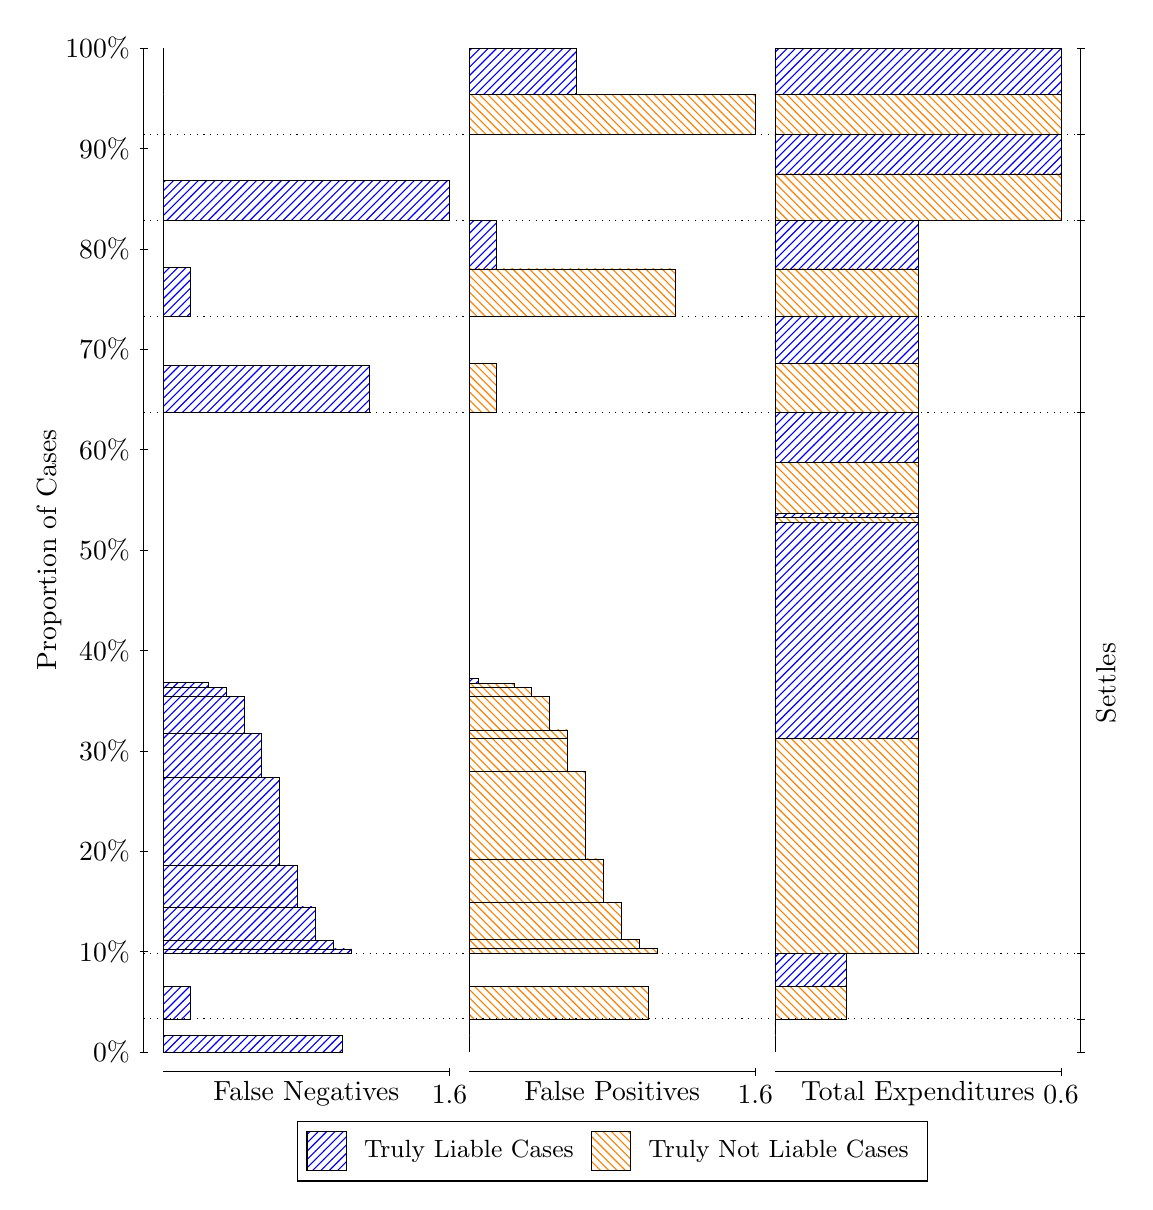
\begin{tikzpicture}
\draw[black, very thin] (1.5,1.75) -- (1.5,14.5);
\node[rotate=90, anchor=center] at (0.3, 8.125) {Proportion of Cases};
\draw[black, very thin] (1.45,1.75) -- (1.55,1.75);
\node[anchor=east] at (1.45, 1.75) {0\%};
\draw[black, very thin] (1.45,3.025) -- (1.55,3.025);
\node[anchor=east] at (1.45, 3.025) {10\%};
\draw[black, very thin] (1.45,4.3) -- (1.55,4.3);
\node[anchor=east] at (1.45, 4.3) {20\%};
\draw[black, very thin] (1.45,5.575) -- (1.55,5.575);
\node[anchor=east] at (1.45, 5.575) {30\%};
\draw[black, very thin] (1.45,6.85) -- (1.55,6.85);
\node[anchor=east] at (1.45, 6.85) {40\%};
\draw[black, very thin] (1.45,8.125) -- (1.55,8.125);
\node[anchor=east] at (1.45, 8.125) {50\%};
\draw[black, very thin] (1.45,9.4) -- (1.55,9.4);
\node[anchor=east] at (1.45, 9.4) {60\%};
\draw[black, very thin] (1.45,10.675) -- (1.55,10.675);
\node[anchor=east] at (1.45, 10.675) {70\%};
\draw[black, very thin] (1.45,11.95) -- (1.55,11.95);
\node[anchor=east] at (1.45, 11.95) {80\%};
\draw[black, very thin] (1.45,13.225) -- (1.55,13.225);
\node[anchor=east] at (1.45, 13.225) {90\%};
\draw[black, very thin] (1.45,14.5) -- (1.55,14.5);
\node[anchor=east] at (1.45, 14.5) {100\%};

\draw[black, very thin] (13.4,1.75) -- (13.4,14.5);
\draw[black, very thin] (13.35,1.75) -- (13.45,1.75);
\node[anchor=west] at (13.35, 1.75) {};
\draw[black, very thin] (13.35,2.1699) -- (13.45,2.1699);
\node[anchor=west] at (13.35, 2.1699) {};
\draw[black, very thin] (13.35,3.003) -- (13.45,3.003);
\node[anchor=west] at (13.35, 3.003) {};
\draw[black, very thin] (13.35,9.87) -- (13.45,9.87);
\node[anchor=west] at (13.35, 9.87) {};
\draw[black, very thin] (13.35,11.091) -- (13.45,11.091);
\node[anchor=west] at (13.35, 11.091) {};
\draw[black, very thin] (13.35,12.314) -- (13.45,12.314);
\node[anchor=west] at (13.35, 12.314) {};
\draw[black, very thin] (13.35,13.407) -- (13.45,13.407);
\node[anchor=west] at (13.35, 13.407) {};
\draw[black, very thin] (13.35,14.5) -- (13.45,14.5);
\node[anchor=west] at (13.35, 14.5) {};

\draw[black, very thin, pattern color=blue, pattern=north east lines] (1.75,1.75) rectangle (4.0208,1.96);
\draw[black, very thin, pattern color=orange, pattern=north west lines] (1.75,1.96) rectangle (1.75,2.1699);
\draw[black, very thin, pattern color=blue, pattern=north east lines] (1.75,2.1699) rectangle (2.0906,2.5865);
\draw[black, very thin, pattern color=orange, pattern=north west lines] (1.75,2.5865) rectangle (1.75,3.003);
\draw[black, very thin, pattern color=blue, pattern=north east lines] (1.75,3.003) rectangle (4.1344,3.0583);
\draw[black, very thin, pattern color=blue, pattern=north east lines] (1.75,3.0583) rectangle (3.9073,3.1643);
\draw[black, very thin, pattern color=blue, pattern=north east lines] (1.75,3.1643) rectangle (3.6802,3.5922);
\draw[black, very thin, pattern color=blue, pattern=north east lines] (1.75,3.5922) rectangle (3.4531,4.1208);
\draw[black, very thin, pattern color=blue, pattern=north east lines] (1.75,4.1208) rectangle (3.226,5.2347);
\draw[black, very thin, pattern color=blue, pattern=north east lines] (1.75,5.2347) rectangle (2.999,5.7942);
\draw[black, very thin, pattern color=blue, pattern=north east lines] (1.75,5.7942) rectangle (2.7719,6.2614);
\draw[black, very thin, pattern color=blue, pattern=north east lines] (1.75,6.2614) rectangle (2.5448,6.3795);
\draw[black, very thin, pattern color=blue, pattern=north east lines] (1.75,6.3795) rectangle (2.3177,6.4392);
\draw[black, very thin, pattern color=orange, pattern=north west lines] (1.75,6.4392) rectangle (1.75,9.87);
\draw[black, very thin, pattern color=blue, pattern=north east lines] (1.75,9.87) rectangle (4.3615,10.467);
\draw[black, very thin, pattern color=orange, pattern=north west lines] (1.75,10.467) rectangle (1.75,11.091);
\draw[black, very thin, pattern color=blue, pattern=north east lines] (1.75,11.091) rectangle (2.0906,11.71);
\draw[black, very thin, pattern color=orange, pattern=north west lines] (1.75,11.71) rectangle (1.75,12.314);
\draw[black, very thin, pattern color=blue, pattern=north east lines] (1.75,12.314) rectangle (5.3833,12.817);
\draw[black, very thin, pattern color=orange, pattern=north west lines] (1.75,12.817) rectangle (1.75,13.407);
\draw[black, very thin, pattern color=orange, pattern=north west lines] (1.75,13.407) rectangle (1.75,13.908);
\draw[black, very thin, pattern color=blue, pattern=north east lines] (1.75,13.908) rectangle (1.75,14.5);
\draw[black, very thin, pattern color=orange, pattern=north west lines] (5.6333,1.75) rectangle (5.6333,1.96);
\draw[black, very thin, pattern color=blue, pattern=north east lines] (5.6333,1.96) rectangle (5.6333,2.1699);
\draw[black, very thin, pattern color=orange, pattern=north west lines] (5.6333,2.1699) rectangle (7.9042,2.5865);
\draw[black, very thin, pattern color=blue, pattern=north east lines] (5.6333,2.5865) rectangle (5.6333,3.003);
\draw[black, very thin, pattern color=orange, pattern=north west lines] (5.6333,3.003) rectangle (8.0177,3.0629);
\draw[black, very thin, pattern color=orange, pattern=north west lines] (5.6333,3.0629) rectangle (7.7906,3.18);
\draw[black, very thin, pattern color=orange, pattern=north west lines] (5.6333,3.18) rectangle (7.5635,3.6449);
\draw[black, very thin, pattern color=orange, pattern=north west lines] (5.6333,3.6449) rectangle (7.3365,4.2011);
\draw[black, very thin, pattern color=orange, pattern=north west lines] (5.6333,4.2011) rectangle (7.1094,5.3104);
\draw[black, very thin, pattern color=orange, pattern=north west lines] (5.6333,5.3104) rectangle (6.8823,5.7341);
\draw[black, very thin, pattern color=orange, pattern=north west lines] (5.6333,5.7341) rectangle (6.8823,5.8397);
\draw[black, very thin, pattern color=orange, pattern=north west lines] (5.6333,5.8397) rectangle (6.6552,6.2692);
\draw[black, very thin, pattern color=orange, pattern=north west lines] (5.6333,6.2692) rectangle (6.4281,6.377);
\draw[black, very thin, pattern color=orange, pattern=north west lines] (5.6333,6.377) rectangle (6.201,6.4338);
\draw[black, very thin, pattern color=blue, pattern=north east lines] (5.6333,6.4338) rectangle (5.7469,6.4934);
\draw[black, very thin, pattern color=blue, pattern=north east lines] (5.6333,6.4934) rectangle (5.6333,9.87);
\draw[black, very thin, pattern color=orange, pattern=north west lines] (5.6333,9.87) rectangle (5.974,10.493);
\draw[black, very thin, pattern color=blue, pattern=north east lines] (5.6333,10.493) rectangle (5.6333,11.091);
\draw[black, very thin, pattern color=orange, pattern=north west lines] (5.6333,11.091) rectangle (8.2448,11.694);
\draw[black, very thin, pattern color=blue, pattern=north east lines] (5.6333,11.694) rectangle (5.974,12.314);
\draw[black, very thin, pattern color=orange, pattern=north west lines] (5.6333,12.314) rectangle (5.6333,12.903);
\draw[black, very thin, pattern color=blue, pattern=north east lines] (5.6333,12.903) rectangle (5.6333,13.407);
\draw[black, very thin, pattern color=orange, pattern=north west lines] (5.6333,13.407) rectangle (9.2667,13.908);
\draw[black, very thin, pattern color=blue, pattern=north east lines] (5.6333,13.908) rectangle (6.9958,14.5);
\draw[black, very thin, pattern color=orange, pattern=north west lines] (9.5167,1.75) rectangle (9.5167,1.96);
\draw[black, very thin, pattern color=blue, pattern=north east lines] (9.5167,1.96) rectangle (9.5167,2.1699);
\draw[black, very thin, pattern color=orange, pattern=north west lines] (9.5167,2.1699) rectangle (10.425,2.5865);
\draw[black, very thin, pattern color=blue, pattern=north east lines] (9.5167,2.5865) rectangle (10.425,3.003);
\draw[black, very thin, pattern color=orange, pattern=north west lines] (9.5167,3.003) rectangle (11.333,5.7341);
\draw[black, very thin, pattern color=blue, pattern=north east lines] (9.5167,5.7341) rectangle (11.333,8.4781);
\draw[black, very thin, pattern color=orange, pattern=north west lines] (9.5167,8.4781) rectangle (11.333,8.535);
\draw[black, very thin, pattern color=blue, pattern=north east lines] (9.5167,8.535) rectangle (11.333,8.5903);
\draw[black, very thin, pattern color=orange, pattern=north west lines] (9.5167,8.5903) rectangle (11.333,9.2332);
\draw[black, very thin, pattern color=blue, pattern=north east lines] (9.5167,9.2332) rectangle (11.333,9.87);
\draw[black, very thin, pattern color=orange, pattern=north west lines] (9.5167,9.87) rectangle (11.333,10.493);
\draw[black, very thin, pattern color=blue, pattern=north east lines] (9.5167,10.493) rectangle (11.333,11.091);
\draw[black, very thin, pattern color=orange, pattern=north west lines] (9.5167,11.091) rectangle (11.333,11.694);
\draw[black, very thin, pattern color=blue, pattern=north east lines] (9.5167,11.694) rectangle (11.333,12.314);
\draw[black, very thin, pattern color=orange, pattern=north west lines] (9.5167,12.314) rectangle (13.15,12.903);
\draw[black, very thin, pattern color=blue, pattern=north east lines] (9.5167,12.903) rectangle (13.15,13.407);
\draw[black, very thin, pattern color=orange, pattern=north west lines] (9.5167,13.407) rectangle (13.15,13.908);
\draw[black, very thin, pattern color=blue, pattern=north east lines] (9.5167,13.908) rectangle (13.15,14.5);
\draw[black, dotted] (1.5,2.1699) -- (13.4,2.1699);
\draw[black, dotted] (1.5,3.003) -- (13.4,3.003);
\draw[black, dotted] (1.5,9.87) -- (13.4,9.87);
\draw[black, dotted] (1.5,11.091) -- (13.4,11.091);
\draw[black, dotted] (1.5,12.314) -- (13.4,12.314);
\draw[black, dotted] (1.5,13.407) -- (13.4,13.407);
\draw[black, very thin] (1.75,1.5) -- (5.3833,1.5);
\node[anchor=north] at (3.5667, 1.5) {False Negatives};
\draw[black, very thin] (5.3833,1.45) -- (5.3833,1.55);
\node[anchor=north] at (5.3833, 1.45) {1.6};

\draw[black, very thin] (5.6333,1.5) -- (9.2667,1.5);
\node[anchor=north] at (7.45, 1.5) {False Positives};
\draw[black, very thin] (9.2667,1.45) -- (9.2667,1.55);
\node[anchor=north] at (9.2667, 1.45) {1.6};

\draw[black, very thin] (9.5167,1.5) -- (13.15,1.5);
\node[anchor=north] at (11.333, 1.5) {Total Expenditures};
\draw[black, very thin] (13.15,1.45) -- (13.15,1.55);
\node[anchor=north] at (13.15, 1.45) {0.6};



\node[black, centered, rotate=90] at (13.72, 6.4365) {Settles};





\draw (7.449999999999999,1.5) node[draw=none] (baseCoordinate) {};
\begin{scope}[align=center]
        \matrix[scale=0.5, draw=black, below=0.5cm of baseCoordinate, nodes={draw}, column sep=0.1cm]{
            \node[rectangle, draw, minimum width=0.5cm, minimum height=0.5cm, pattern=north east lines, pattern color=blue] {}; &
            \node[draw=none, font=\small] (B) {Truly Liable Cases}; &
            \node[rectangle, draw, minimum width=0.5cm, minimum height=0.5cm, pattern=north west lines, pattern color=orange] {}; &
            \node[draw=none, font=\small] (B) {Truly Not Liable Cases}; \\
            };
\end{scope}

\end{tikzpicture}
\end{document}